\subsection{What is a Tree ?}
\begin{tcolorbox}[title=Tree definition,coltitle =black,fonttitle=\large\bfseries,colback=green!5!white,colframe=green!75!black]
	A non-linear data structure where nodes are organized in a hierarchy.
\end{tcolorbox}

\subsubsection{Basic Terminologies}
\begin{figure}[H]
	\centering
	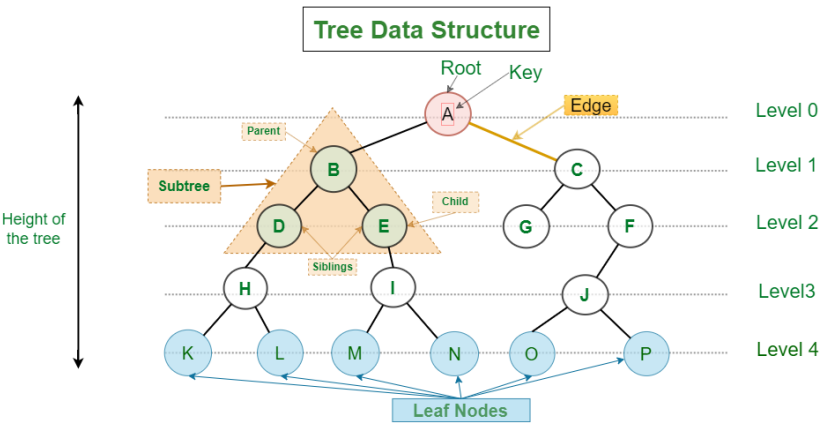
\includegraphics[width=1\textwidth]{figures/tree}
	\caption{Tree terminologies}
\end{figure}
\begin{itemize}
	\item Node: A basic unit of a tree containing data and links to its children.
	\item Root: The topmost node of the tree. There is only one root in a tree.
	\item Parent: A node that has one or more child nodes.
	\item Child: A node that descends from another node (its parent).
	\item Leaf: A node that has no children.
	\item Internal Node: A node that has at least one child.
	\item Edge: A link between a parent and a child node.
	\item Path: A sequence of nodes and edges connecting a node with a descendant.
	\item Subtree: A tree formed by a node and its descendants.
	\item Level (or Depth): The number of edges from the root to the node (root is level 0).
	\item Height of a Node: The number of edges on the longest path from the node to a leaf.
	\item Height of tree: The height of the root node.
	\item Degree of Node: The number of children of a node.
\end{itemize}

\subsection{Tree Implementation}
\begin{lstlisting}[language=python, caption={Defining Tree Node}]
	class TreeNode:
		def __init__(self, data):
			self.data = data
			self.children = []
			self.parent = None
	
		def add_child(self, child):
			child.parent = self
			self.children.append(child)
	
		def get_level(self): #to get level of each node
			level =0
			p = self.parent
			while p:
				level += 1
				p = p.parent
	
			return level
		def print_tree(self):
			space = ' ' * self.get_level() * 3
			prefix = space + '|__' if self.parent else ''
			print(prefix + self.data)#add prefix
			if self.children:
				for child in self.children:
					child.print_tree()
\end{lstlisting}

\begin{lstlisting}[language=python, caption={Example of creating a Tree from Nodes}]
	def create_tree():
		a_node = TreeNode("A")
		b_node = TreeNode("B")
		c_node = TreeNode("C")
		d_node = TreeNode("D")
		e_node = TreeNode("E")
		f_node = TreeNode("F")
		g_node = TreeNode("G")
	
		a_node.add_child(b_node)
		a_node.add_child(c_node)
		
		b_node.add_child(d_node)
		b_node.add_child(e_node)
	
		c_node.add_child(f_node)
		c_node.add_child(g_node)
		return a_node
		
		tree = create_tree()
		tree.print_tree()
\end{lstlisting}

Expected Result:
\begin{figure}[H]
	\centering
	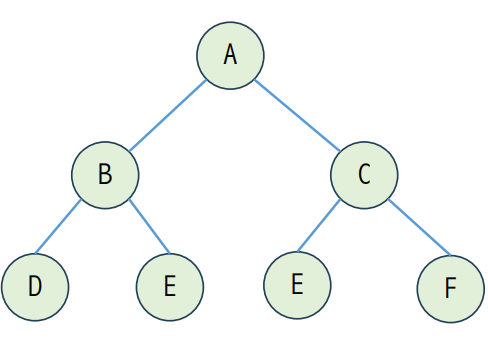
\includegraphics[width=0.7\textwidth]{figures/expected-tree}
	\caption{Expected Tree}
	\label{fig:expected-tree}
\end{figure}

\subsection{Tree applications}
\subsubsection{Storing naturally hierarchical data}
Data is organised hierarchically using trees.
\begin{figure}[H]
		\centering
		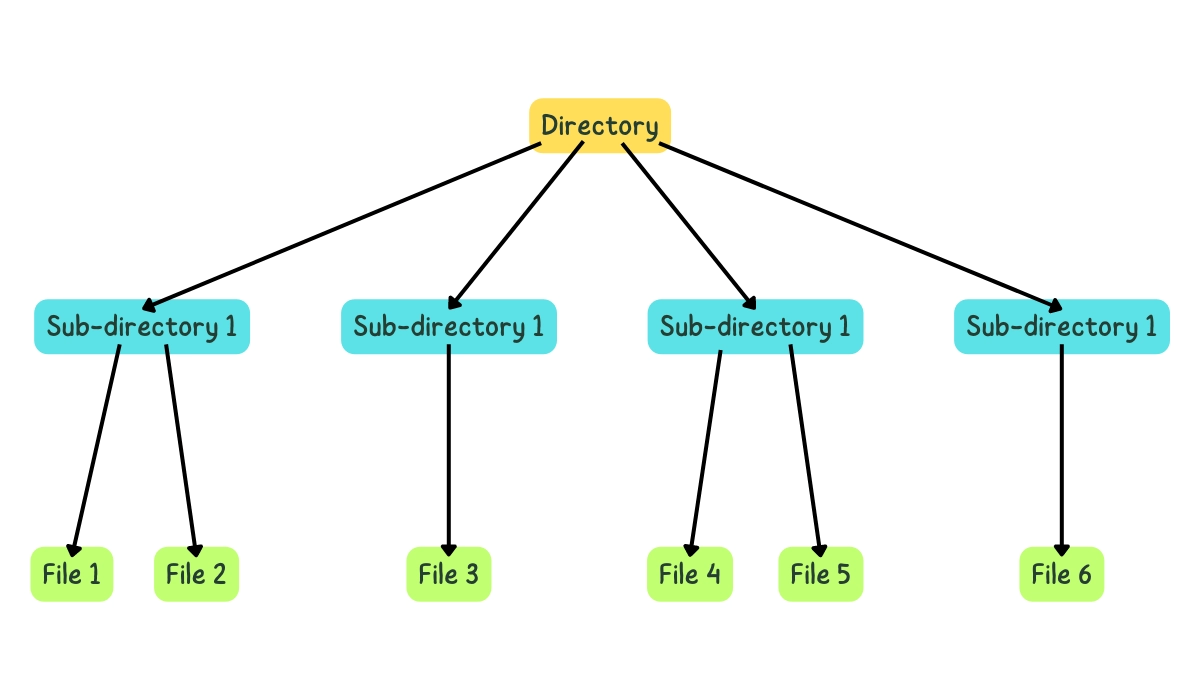
\includegraphics[width=0.85\textwidth]{figures/tree-app-1}
		\caption{Computer's file system}
		\label{fig:tree-app-1}
\end{figure}
\begin{figure}[H]
	\centering
	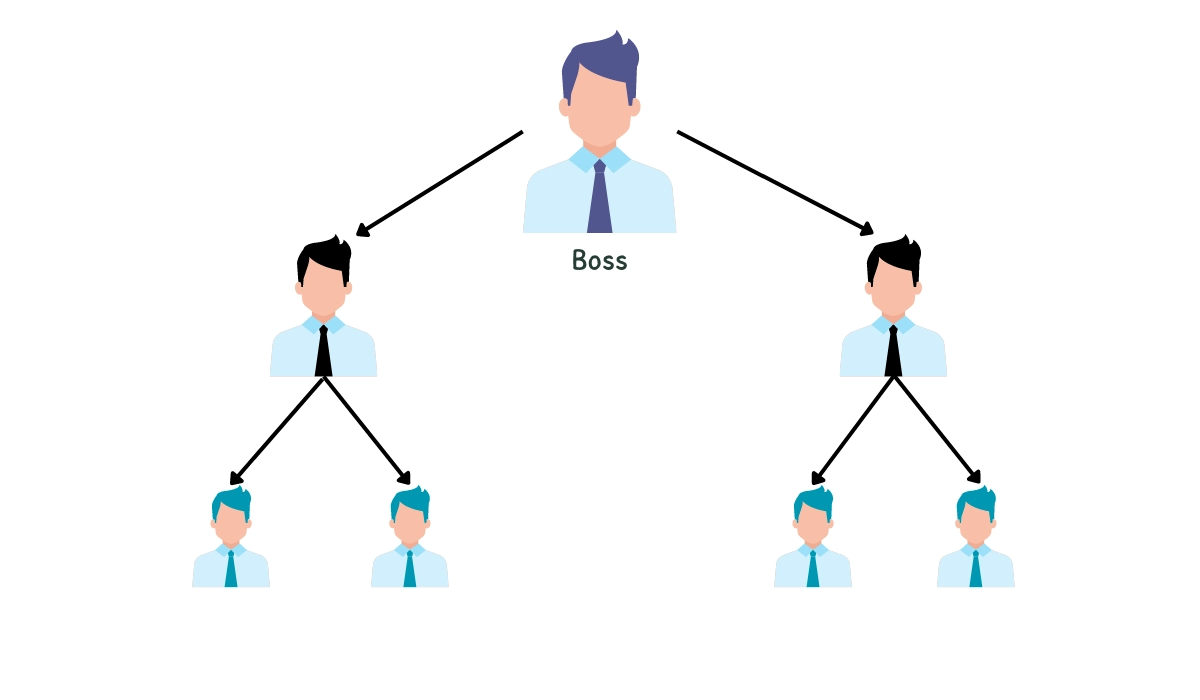
\includegraphics[width=0.85\textwidth]{figures/tree-app-2}
	\caption{Organisational structure}
	\label{tree-app-2}
\end{figure}
\subsubsection{ML-AI: Decision Tree/K-D Tree}
\begin{tcolorbox}[title=Decision trees,coltitle =black,fonttitle=\large\bfseries,colback=green!5!white,colframe=green!75!black]
In machine learning and data mining, decision trees are represented by tree data structures. Each node in a decision tree represents a choice or a feature, and the child nodes represent the feature's possible outcomes or values.
\end{tcolorbox}
{\large Example 1:} A student set a rule for himself about whether to study or play. If there are more than two days left until the day, he will go out. If there are less than two days left and there is a football match tonight, he will sing at his friend's house and watch the match together. He will only study in other cases.\\

\begin{figure}[H]
	\begin{minipage}[T]{0.45\textwidth}
		\raggedright
		The yellow ellipse represents the decision that needs to be made. This decision depends on the answers to the questions in the gray rectangles. Based on the answers, the final decision is given in the green (play) and red (study) circles.
	\end{minipage}
	\hfill
	\begin{minipage}[T]{0.4\textwidth}
		\centering
		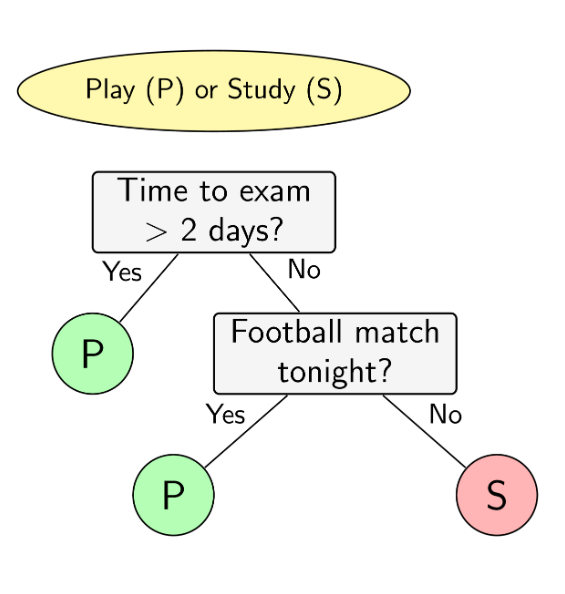
\includegraphics[width=\linewidth]{figures/decision-tree-ex1}
		\caption{Example of decision making using a Tree}
	\end{minipage}
\end{figure}

{\large Classification using Decision tree:} In the following example, the task is to find a simple boundary that separates these two classes. In other words, this is a classification problem, we need to build a classifier to decide which class a new data point belongs to. If a point has the first component, x1, less than the threshold, t1, we immediately decide that it belongs to the green class. In addition, if the second component, x2, is greater than the threshold, t2, we decide that it also belongs to the green class. Next, if the first component, x1, is greater than threshold, t3, we decide that it belongs to the green class. Points that do not satisfy the above conditions are classified as red class.

\begin{figure}[H]
	\begin{minipage}{0.45\textwidth}
		\centering
		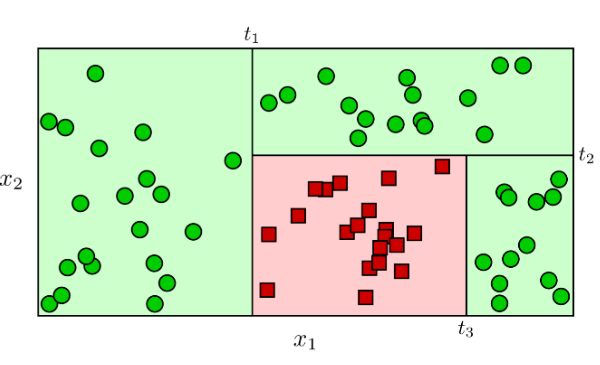
\includegraphics[width=\linewidth]{figures/decision-tree-classification-1}
		\caption{(a)}
	\end{minipage}
	\hfill
	\begin{minipage}{0.45\textwidth}
		\centering
		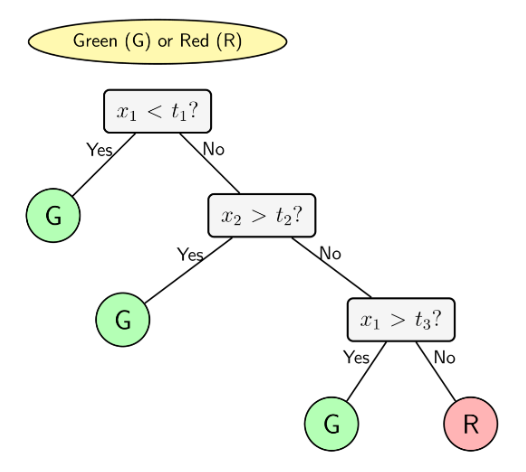
\includegraphics[width=\linewidth]{figures/decision-tree-classification-2}
		\caption{(b)}
	\end{minipage}
\end{figure}

\subsection{Types of Trees}
\subsubsection{Binary Tree}
A binary tree is a tree data structure where each node has at most two children. These two children are usually referred to as the left child and right child. It is widely used in applications such as binary search trees and heaps.

\begin{figure}[H]
	\centering
	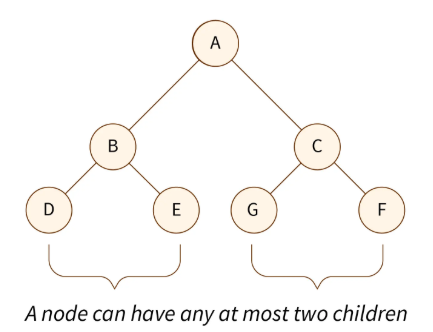
\includegraphics[width=0.6\textwidth]{figures/binary-tree}
	\caption{Binary Tree}
	\label{fig:bitree}
\end{figure}

\subsubsection{Ternary Tree}
It is a type of tree data structure where each node can have a maximum of three child nodes., commonly referred to as "left", "mid", and "right".
\begin{figure}[H]
	\centering
	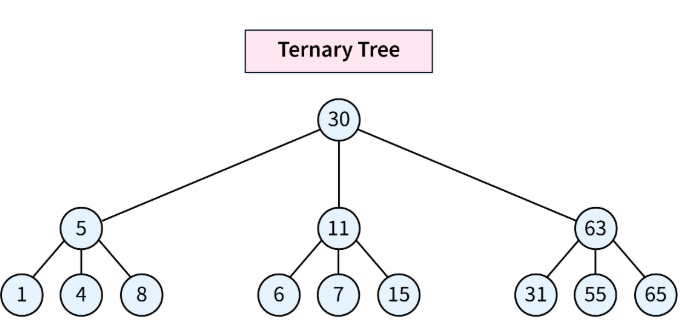
\includegraphics[width=0.75\textwidth]{figures/ternary-tree}
	\caption{Ternary Tree}
	\label{fig:tertree}
\end{figure}

\subsubsection{N-ary Tree}
An N-ary Tree, also called a Generic Tree, is a type of tree data structure. In an N-ary tree, each node holds data records and references to its children. It prohibits duplicate references among its children. \\
Key features of an N-ary tree:\\
\begin{itemize}
	\item Each node can have multiple children.
	\item The exact number of children for each node is not predetermined and may vary.
\end{itemize}

\begin{figure}[H]
	\centering
	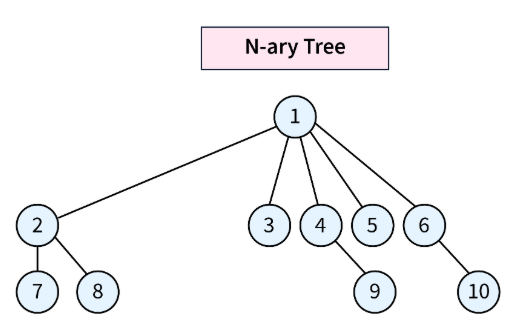
\includegraphics[width=0.65\textwidth]{figures/n-ary-tree}
	\caption{N-ary Tree}
	\label{fig:nary}
\end{figure}

\subsection{Algorithms on Trees}
\subsubsection{Traversal of Binary Tree}
\begin{tcolorbox}[title=Traversal of Binary Tree,coltitle =black,fonttitle=\large\bfseries,colback=green!5!white,colframe=green!75!black]
	Traversal on a tree refers to the process of visiting (checking and/or updating) each node in a tree data structure, exactly once, in a systematic way.
	\begin{itemize}
		\item Breadth first search: Explores all the nodes in a tree at the current depth before
		moving on to the vertices at the next depth level.
		\item Depth first search: The algorithm starts at the root node and explores as far as possible along each branch before backtracking
	\end{itemize}
\end{tcolorbox}

\begin{figure}[H]
	\begin{minipage}{0.45\textwidth}
		\centering
		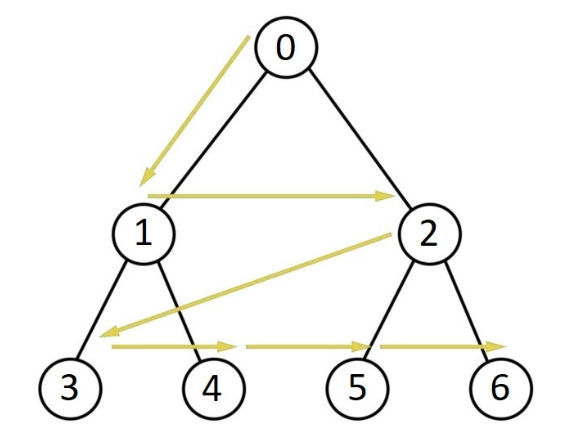
\includegraphics[width=\linewidth]{figures/bfs}
		\caption{BFS}
	\end{minipage}
	\hfill
	\begin{minipage}{0.45\textwidth}
		\centering
		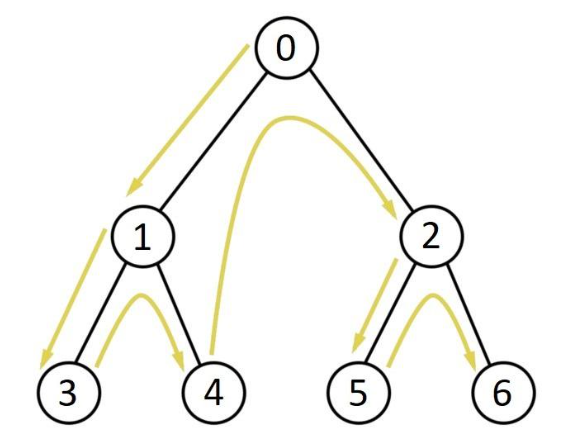
\includegraphics[width=\linewidth]{figures/dfs}
		\caption{DFS}
	\end{minipage}
\end{figure}


	